% !TeX root = ../main.tex
\chapter{System Test Results and Project Summary}
\label{chap:test-results}

This chapter describes the final test of the Multi-Rail Isolated Power Supply Monitoring System and gives the assessment of the entire capstone project. The chapter is split in two parts according to the final project assignment. Part A describes the execution of the system test plan developed in the previous chapter, gives the results of the test and provides conclusions based on these results. Part B evaluates the completed project in terms of scope, schedule, budget and stakeholder expectations.

\section{Part A: Test Plan and Results}
\label{sec:part-a-test-results}

The test plan developed in in the previous chapter was performed after completion of hardware bring-up, firmware development, local display integration, Ethernet communications, and EPICS IOC integration. Testing was done for the whole assembled system instead of the individual circuit blocks in order to assess the interactions between the sensor hardware, Arduino controller, firmware, local display, Ethernet communications, EPICS IOC, and test software.

The final test produced the automated PDF system test report containing acceptance criteria, overall test matrix, rail-by-rail measurement results, error plots, operator observations, detailed system test checklist, completion criteria, and engineering justification for the selected tolerances. The complete generated report is attached at the end of Part A.

\subsection{Test Execution}

Tests were conducted on each of the six monitored power supply rails:

\begin{itemize}
	\item +5VA,
	\item +5VB,
	\item +5~V,
	\item $-$5~V,
	\item +15~V, and
	\item $-$15~V.
\end{itemize}

A Rigol programmable electronic load was used to set multiple load cases on each rail. During each test point, the external reference voltage and current were compared with the corresponding measurements reported by the EPICS IOC. The local GIGA display was also observed to check rail identity, polarity, measurements updates, limits state and communication state.

The +5VA and +5VB channels were tested at approximately 0~A, 1~A, and 2~A. The other +5~V, $-$5~V, +15~V, and $-$15~V channels were tested at approximately 0~A, 0.5~A, and 1~A. The result was multiple operating points for every monitored rail instead of checking the system under a single load.

The Python test software automated the acquisition of the EPICS values, measurement error calculation, application of acceptance limits, data saving and generation of the final PDF report. When operator observation was required, such as the verification of the information displayed on the local display, the result was recorded in the system test checklist.

\subsection{Acceptance Criteria}

The acceptance criteria formulated in the previous chapter were kept for the final system test. The main electrical acceptance criteria were:

\begin{itemize}
	\item The IOC voltage measurements must agree with the external reference within $\pm2\%$ across the whole test range.
	\item The IOC current measurements must agree with the external reference within $\pm5\%$ across the whole intended range.
	\item For low current values, the bigger of the percentage tolerance and absolute error floor is used. The absolute floor is 25~mA for the 39~m$\Omega$ channels and 20~mA for the 50~m$\Omega$ channels.
	\item Positive and negative rail voltages must be represented correctly in terms of polarity.
	\item The local-display and EPICS values must represent the same underlying measurement within the display resolution and rounding.
	\item Programmable voltage and current limits must work correctly in terms of assertion and de-assertion.
	\item Persistent settings must survive the removal and restoration of the controller power.
	\item Local monitoring must operate during network interruption and the EPICS communication must be restored after Ethernet recovery.
\end{itemize}

These criteria provided the measurable limits by which the completed prototype could be evaluated instead of the subjective judgment that the system appeared to be working.

\subsection{System Test Results}

The system test of the completed system produced the overall result of \textbf{PASS}. All six rail measurement tests passed, and each of the twelve system level tests formulated in Chapter 6 also passed.

Table~\ref{tab:system-test-results} summarizes the final system test disposition.

\begin{table}[htbp]
	\centering
	\caption{Final system test results.}
	\label{tab:system-test-results}
	\begin{tabular}{clc}
		\hline
		\textbf{Test ID} & \textbf{Test} & \textbf{Result} \\
		\hline
		ST-01 & Power On and Initialization & PASS \\
		ST-02 & Rail Identification & PASS \\
		ST-03 & Voltage Accuracy & PASS \\
		ST-04 & Current Accuracy & PASS \\
		ST-05 & Dynamic Load Response & PASS \\
		ST-06 & Local Display & PASS \\
		ST-07 & EPICS Communications & PASS \\
		ST-08 & Limit / Alarm Operation & PASS \\
		ST-09 & Persistent Settings & PASS \\
		ST-10 & Communication Recovery & PASS \\
		ST-11 & Repeatability & PASS \\
		ST-12 & End-To-End Demonstration & PASS \\
		\hline
	\end{tabular}
\end{table}

Also, the latest accepted attempt for each individual rail passed, as summarized in Table~\ref{tab:rail-results}.

\begin{table}[htbp]
	\centering
	\caption{Final rail measurement results.}
	\label{tab:rail-results}
	\begin{tabular}{ccc}
		\hline
		\textbf{Rail} & \textbf{IOC Channel} & \textbf{Result} \\
		\hline
		+5VA  & 5VA  & PASS \\
		+5VB  & 5VB  & PASS \\
		+5~V  & P5V  & PASS \\
		$-$5~V  & M5V  & PASS \\
		+15~V & P15V & PASS \\
		$-$15~V & M15V & PASS \\
		\hline
	\end{tabular}
\end{table}

All required voltage samples satisfied the system-level voltage accuracy criterion, and all required current samples satisfied the current accuracy criterion, including the low current absolute tolerance when applicable. Both negative voltage channels reported the correct negative voltage polarity while preserving the positive current magnitude convention used by the firmware.

Dynamic load testing also passed on all six channels. The changes in electronic load current were reflected on the local display and on the corresponding EPICS process variables, and none of the channels became unresponsive during the load sweeps.

Local display testing confirmed that all six channel identifications, voltage values, current values, programmed limits, status indication, and communication information were visible and corresponded to the appropriate physical rail. All local display observations recorded during the test passed for every monitored channel.

EPICS communication testing confirmed that the IOC connected to the Arduino TCP server and that the required voltage and current process variables for all six rails were connected and updated. The load changes were observed by EPICS for both positive and negative channels, confirming the proper operation of the complete measurement and communication chain.

Limit testing confirmed that the system reacted correctly when the applied measurement crossed the programmed threshold. Both the local display and the EPICS status changed when the threshold was exceeded and returned to normal when the measurement came back inside the configured limits.

Persistent settings testing was performed by changing known user-adjustable settings, removing power from the monitoring electronics, restoring power, and comparing the recovered values with the values stored prior to the power cycling. The stored values were recovered correctly.

Communication recovery testing was performed by interrupting Ethernet communication while the monitor was running. The local GIGA display continued to operate during the interruption. After Ethernet was restored, the communication with the IOC was recovered without firmware reprogramming and the EPICS process variables started to update again with the valid values.

Repeatability testing was also passed. The measurements repeated at selected operating points, including after the power cycle, were within the established acceptance limits, and no intermittent sensor or communication problems were observed.

Finally, the end-to-end demonstration confirmed simultaneous operation of the complete hardware, firmware, local display, network interface, EPICS IOC, Phoebus interface and automated test software. The change of the load on the monitored channel produced the expected result locally and remotely without system-level problems.

\subsection{Conclusions and Results}

The final test results confirm that the completed prototype satisfied the main functional and measurement requirements established for the project. All twelve system level tests passed and all six monitoring channels passed their final voltage and current verification.

The voltage and current tests are especially important since they give the quantitative proof that the monitor implements its intended measurement function. The testing was performed at multiple operating points on each channel instead of the single nominal load case. This gives the higher confidence that the measurement system works properly across the intended range of loads.

The test results also confirmed the functions that cannot be confirmed by measurement accuracy alone. Correct rail identification and polarity were confirmed, including the two negative voltage channels. The local graphical interface and EPICS interface displayed the same underlying information, programmable limits worked correctly, persistent settings were recovered from the storage, and the network communication was restored after the intentional interruption.

The conclusion regarding the operation of the system in the broad range of temperature, electromagnetic compatibility, vibration, mechanical shock, accelerated aging, and destructive fault conditions cannot be made since these qualification tests were intentionally excluded from the system test plan. The additional measurements are needed to make claims regarding performance under those conditions.

Some of the problems discovered during the board bring-up were fixed before the final system test. They included the SDA polarity problem in the isolated I\textsuperscript{2}C interface, pull-up and signal state problems, and startup sequencing problems. The successful final acceptance test confirms that the corrective modifications were effective and that these earlier development problems did not prevent the completed prototype from passing the final system test.

\subsection{Recommendations and Improvement Opportunities}

Despite the fact that the completed system satisfied the acceptance criteria, some improvements are recommended for the future PCB revision.

The most important hardware improvement is the incorporation of the SDA polarity fix directly in the PCB design. The prototype required the SN74LVC2G04 inverter to correct the SDA signal polarity after the originally installed LTC2945 device variant turned out to be incompatible with the intended isolation interface. The future revision should use the correct LTC2945 variant throughout the design or incorporate the required inversion directly in the schematic and PCB.

All required I\textsuperscript{2}C pull-up resistors and defined logic states should also be incorporated directly in the next PCB revision. It will eliminate the prototype modification and improve the repeatability of assembly and startup.

The firmware initialization can also be made more tolerant of arbitrary power-up sequencing. During the development, the communication could be failed when the controller tried to initialize the sensor before the corresponding isolated rail circuitry was powered. The future firmware revision could periodically retry the unavailable sensors so that the communication is established automatically when the monitored rail is powered.

The per-channel measurement calibration is another potential improvement. The present system calculates the current using the configured current sense resistance. The measurement of the actual resistance or the determination of the calibration factor against the external reference will allow the individual gain correction to be stored for each channel. It will help to reduce the systematic errors caused by the shunt tolerance and allow tighter acceptance limits if the improved measurement accuracy is required.

The additional environmental characterization is also useful if the design is going to be developed beyond the capstone prototype. The testing at multiple ambient temperatures can be used to determine whether the temperature affects the measurement accuracy. EMC testing can determine the susceptibility to and generation of the electromagnetic interference. The long duration testing can be used to detect the intermittent communication, thermal, network or firmware problems that might not occur during the shorter acceptance test.

The automated test system should be retained for the future revisions. Since the raw measurements are saved separately from the report generation, the future hardware or firmware revisions can be tested using the same acceptance procedure and direct comparison between the revisions is possible.

These recommendations represent the refinements in reliability, manufacturability, calibration and qualification and not the changes to the basic architecture. The successful final test proves that the overall system concept is suitable for the further development.

\subsection{Generated System Test Report}
\label{sec:generated-test-report}

The automated System Test Report generated from the final accepted test data is attached below as the permanent part of the project test record. The report contains the detailed rail-by-rail measurements, measurement error plots, system test checklist, acceptance results, and engineering justification for the selected tolerances.

\clearpage

% Requires \usepackage{pdfpages} in the document preamble.
% Change the path below if the PDF is stored in another directory.
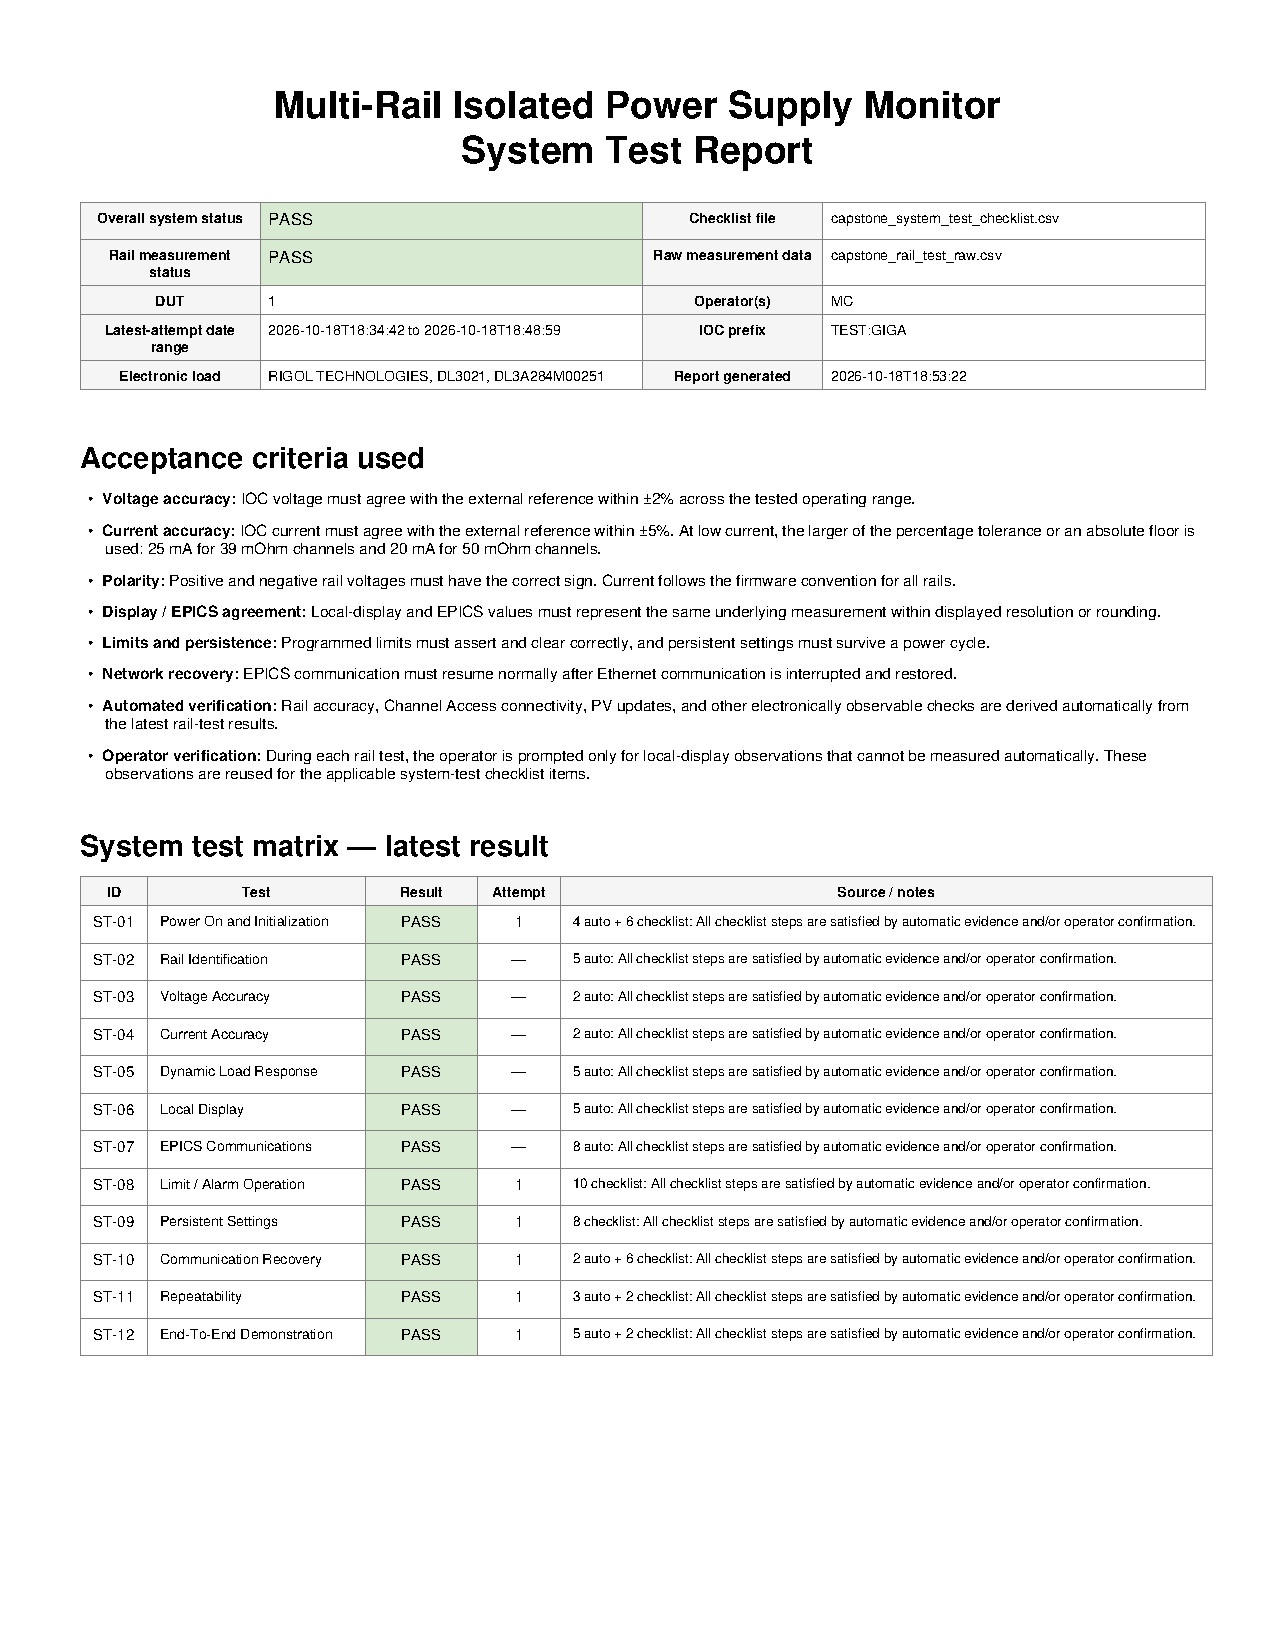
\includepdf[
pages=-,
pagecommand={\thispagestyle{plain}},
fitpaper=true
]{Pictures/capstone_rail_test_report_20261018_185322.pdf}

\clearpage


\section{Part B: Project Summary}
\label{sec:part-b-project-summary}

The final project assessment should take into account not only whether the prototype operates, but also whether the completed capstone fulfilled its original scope, schedule, budget and stakeholder expectations. The completed system and the results of Part A form the basis for this evaluation.

\subsection{Did the Project Meet the Requirements of the Scope?}

The project fulfilled the major requirements of the original project scope.

The completed system provides six independent voltage and current monitoring channels corresponding to +5VA, +5VB, +5~V, $-$5~V, +15~V, and $-$15~V. The high side current sensing is used for each channel while the electrical isolation is preserved between independently referenced monitored supplies and the common controller.

The completed hardware includes the sensor interface, current sense resistors, isolation circuitry, Arduino GIGA controller interface, local display, controller power circuitry and Ethernet interface. The software implementation includes the embedded measurement acquisition, conversion to engineering units, configurable limits, alarm processing, persistent configuration storage, local graphical display, network communication, the EPICS IOC, process variable database records and the Phoebus operator interface.

The final system testing confirmed the correct operation of all six measurement channels, the correct positive and negative voltage representation, programmable limit operation, persistent settings, local display operation, Ethernet communication, EPICS monitoring, communication recovery, repeatability, and end-to-end operation.

The hardware, firmware, IOC files, operator interface files, documentation and other project artifacts were also maintained under revision control as required by the project scope.

Based on the completed implementation and the final system test results, the capstone project is therefore considered to have fulfilled its technical scope.

\subsection{Was the Project Completed on Time?}

The project was completed within the planned capstone schedule.

The original project plan distributed the development across the eight week ET410 planning phase and the following eight week ET450 implementation phase, with the completed system expected to be ready for demonstration by Week 7 of ET450. The final automated system test was completed on October 18, 2026, giving the completed and verified system before the planned final demonstration period.

The project experienced the schedule risk during the hardware bring-up. Troubleshooting of the isolated I\textsuperscript{2}C interface required additional effort after the SDA polarity problem and other communication problems were discovered. The startup sequencing and Ethernet integration also required the troubleshooting that was not anticipated in the initial plan.

These problems consumed the schedule margin, but they were fixed without preventing the completion of the prototype and final system test within the capstone schedule. The project is therefore considered to have fulfilled the schedule requirement.

\subsection{Was the Project Completed Under Budget?}

The project was not completed within the original preliminary hardware budget.

The initial project proposal assumed the material and contingency budget of \$660. This estimate was based on the incomplete information about the detailed component selection, custom PCB layout and final vendor pricing.

After completion of the detailed design and Bill of Materials, the estimated one system hardware purchase cost became \$1,019.03. It includes \$242.36 in the Sensor Board components, \$473.57 for the minimum Sensor Board PCB order, \$180.90 in the Arduino Shield components, and \$122.19 for the minimum Arduino Shield PCB order.

Compared to the original \$660 estimate, the final documented hardware purchase estimate is \$359.03 higher than the preliminary budget. The additional cost is due to a better definition of the component as well as the minimum order cost related to the fabrication of the custom PCBs.

Thus, the cost estimate was good to use as a preliminary cost estimate value but did not provide enough cost to build a complete prototype of a custom PCB. The project should be considered above the original hardware budget.

This cost comparison concerns only the documented prototype hardware cost. Laboratory test equipment, software, labor, shipping, taxes, enclosure hardware, cabling and any other items not included into the project cost analysis are not included into this cost comparison.

\subsection{Did the Quality and Performance Meet Stakeholder Expectations?}

The quality and performance of the completed prototype met the expectations set for the capstone project.

The main project stakeholders are the project developer, the course instructor and the potential technical users of the system. The best evidence of system quality is the completed acceptance test. All twelve expected system tests were completed successfully, all six monitored rails passed the voltage and current check, and the complete system demonstration was successful without any system failures.

The prototype showed the capability to collect isolated voltage and current measurements, display the data locally, compare the data with configurable limits, keep the configuration after the restart, send the data via Ethernet, support the EPICS integration, present the data using Phoebus and to restore the operation after the network connection interruption.

The project provided the possibility to develop the repeatable automated test procedure instead of using the subjective one. The raw data were saved and used for the creation of a test report including the measurement data, pass/fail result and the test evidence. It improves the confidence in the final result and allows assessing future revisions of the hardware.

The prototype still includes some features which should be improved in the future production revision of the design, such as SDA inverter modification, modified implementation of the I\textsuperscript{2}C pull-up, correct startup sequence and the possible implementation of the per-channel calibration. They do not prevent the prototype from meeting the acceptance criteria, but may influence the manufacturability and further improvements of the design.

Based on the final test results, the completed project can be stated to meet the stakeholder expectations in terms of functionality and performance.

\subsection{Overall Project Assessment}

The Multi-Rail Isolated Power Supply Monitoring System successfully passed the full project cycle including the project definition and preliminary design, custom hardware development, firmware implementation, network and EPICS integration, board bring-up, troubleshooting and system verification.

The biggest challenges of the project were related to the hardware integration instead of development of the individual functions of the system. The troubleshooting of the isolated I\textsuperscript{2}C interface showed the necessity to check the component version, polarity, pull-up requirement, signal states and startup behavior in the physical implementation. These issues were found by the measurements, fixed and retested in the final system tests.

The completed prototype met the defined project scope, completed in the required time and met the final technical acceptance criteria. Although the project cost exceeds the original preliminary hardware budget, the detailed cost estimation provides more realistic basis for the estimation of the cost of prototype and future production revision.

Finally, the successful completion of the system test showed that the hardware, embedded firmware, local user interface, Ethernet communication, EPICS IOC, Phoebus interface and the automated test software work as the integrated system. Thus, the project successfully reached the main goal of development and demonstration of the functioning six-channel isolated power supply monitoring system.